\documentclass[twocolumn,tighten,times]{aastex62}


\usepackage{amsmath}
\usepackage{nicefrac}

\usepackage{xspace} %to preserve spaces following a control word




%elements
\newcommand{\iso}[2]{\ensuremath{\mathrm{{^{#2}}#1}}} % Isotopes, e.g. \iso{c}{12}
\newcommand{\abun}[2]{\ensuremath{X(\mathrm{{^{#2}}#1}})} % Isotope abundance 

% units 
\newcommand{\msun}{\ensuremath{\mathrm{\,M_\odot}}} % Msol 
\newcommand{\rsun}{\ensuremath{\mathrm{\,R_\odot}}} % Rsol
\newcommand{\lsun}{\ensuremath{\mathrm{\,L_\odot}}} % Lsol
\newcommand{\zsun}{\ensuremath{\mathrm{\,Z_\odot}}} % Solar metallicity
\newcommand{\ledd}{\ensuremath{\mathrm{\,L_{Edd}}}} % Eddington luminosity
\newcommand{\mdotsun}{\ensuremath{\mathrm{\,M_{\odot}\,yr^{-1}}}} % solar masses per yr
\newcommand{\erg}{\,\ensuremath{\mathrm{erg}}} %erg 
\newcommand{\ergs}{\ensuremath{\mathrm{\,erg\,s^{-1}}}} %ergs per sec  
\newcommand{\secsec}{\ensuremath{\mathrm{\,s\,s^{-1}}}} %sec per sec
\newcommand{\kms}{\ensuremath{\mathrm{\,km\,s^{-1}}}} %km per sec
\newcommand{\ms}{\ensuremath{\mathrm{\,m\,s^{-1}}}}%m per sec
\newcommand{\dmu}{\ensuremath{\mathrm{\,pc\,cm^{-3}}}} %DM units 
\newcommand{\denu}{\ensuremath{\mathrm{\,g\,cm^{-3}}}} %density units 

%quantities
\newcommand{\tc}{\ensuremath{T_{\mathrm{c}}}} % Central temperature 
\newcommand{\logtc}{\ensuremath{\log_{10} (T_{\mathrm{c}}/{\mathrm{K})}}} %log central temperature
\newcommand{\logt}{\ensuremath{\log_{10} T}} % Log temperature
\newcommand{\logl}{\ensuremath{\log_{10} (L/\lsun)}} % Log Luminosity
\newcommand{\rhoc}{\ensuremath{\rho_{\mathrm{c}}}} % Central density 
\newcommand{\logrhoc}{\ensuremath{\log_{10} (\rho_{\mathrm{c}}/ \mathrm{g\,cm^{-3}})}} % Log central density
\newcommand{\logrho}{\ensuremath{\log \rho}} % Log  density
\newcommand{\teff}{\ensuremath{T_{\mathrm{eff}}}} % Effective temperature 
\newcommand{\logteff}{\ensuremath{\log_{10} (T_{\mathrm{eff}} /\mathrm{K})}} % Log effective temperature
\newcommand{\mch}{\ensuremath{M_{\mathrm{Ch}}}} % Chandrasekhar mass
\newcommand{\mdot}{\ensuremath{\dot{M}}} % Mdot
\newcommand{\pdot}{\ensuremath{\dot{P}}} % Pdot
\newcommand{\rdot}{\ensuremath{\dot{R}}} % Rdot
\newcommand{\ye}{\ensuremath{Y_e}} % Rdot

%Abbreviations
\newcommand{\vdag}{(v)^\dagger} %version
\newcommand\aastex{AAS\TeX} %aastex 
\newcommand\latex{La\TeX} %latex
\newcommand{\mesa}{{\textsc{mesa}}\xspace} %MESA
\newcommand{\ia}{SN\,Ia\xspace} %SN Ia
\newcommand{\ias}{SNe\,Ia\xspace} %SNe Ia 
\newcommand\one{(C)N\lowercase{e}O\xspace} %(C)NeO
\newcommand{\dtd}{\ensuremath{\mathrm{DTD}(t)}}

 
%% figures live in this folder 
\graphicspath{{./}{figures/}}


%\received{January 1, 2018}
%\revised{January 7, 2018}
%\accepted{\today}
\submitjournal{AAS Journals}
\shorttitle{\ias from non-accreting progenitors}
\shortauthors{Antoniadis et al.}


\begin{document}


\title{TYPE Ia SUPERNOVAE FROM NON-ACCRETING PROGENITORS}


\correspondingauthor{John Antoniadis}
\email{janton@mpifr.de}

\author[0000-0002-0786-7307]{John Antoniadis}

\affil{Max-Planck Institut f\"{u}r Radioastronomie, Auf dem H\"{u}gel 69, 53121, Bonn DE}
\affil{Argelander Institut f\"{u}r Astronomie,
Auf dem H\"{u}gel 71, 53121, Bonn DE}

\author[0000-0002-9323-9728]{S. Chanlaridis}
\author{G\"{o}tz Gr\"{a}fener}
\affil{Argelander Institut f\"{u}r Astronomie, 
Auf dem H\"{u}gel 71, 53121, Bonn DE}
\author{Norbert Langer}
\affil{Argelander Institut f\"{u}r Astronomie, 
Auf dem H\"{u}gel 71, 53121, Bonn DE}
\affil{Max-Planck Institut f\"{u}r Radioastronomie, Auf dem H\"{u}gel 69, 53121, Bonn DE}

\begin{abstract}
We study the late evolution of two helium stars with masses of 1.8 and 2.5\,M$_{\odot}$, considering the effects of electron captures, urca cooling. We demostrate that the mass of the core grows steadily and reaches the Chandrasekhar mass limit. Both models avoid electron capture reactions. 
\end{abstract}

\keywords{supernovae: general -- evolution – stars: interiors}

\section{Introduction} \label{sec:intro}
%Type Ia supernovae (\ias) signal the disruption of a star 
%in a thermonuclear explosion. 
%The prompt conversion of $\sim 0.6$\,M$_{\odot}$ of  
%material into iron-peak elements, and the subsequent 
%radioactive decay of $^{56}$Ni ejecta, power a luminous 
%transient able to shine across  cosmological 
%distances \citep[e.g.][]{Arnett:1982}.
%Besides reaching high bolometric luminosities, 
%the bulk of \ia light curves also show remarkable 
%homogeneity in their evolution \citep{Phillips:1993ng}. 
%This makes them unique cosmological distance indicators 
%and valuable tools for probing the expansion history of the Universe %\citep{Riess:1998cb,Perlmutter:1998np}. 
 Despite their central role in Astrophysics and Cosmology, 
 the origin and physics of Type Ia supernova explosions (\ias)
remain uncertain  \citep[][]{Maoz:2013hna}. 
The observed luminosities ($\ge 10^{43}$\ergs) and ejecta velocities  
($ \sim 10^{4}$\kms), imply \iso{Ni}{56}  
masses and kinetic energies of order 
$\sim 0.6$\msun\ and $\sim 10^{51}$\erg\ respectively. 
 These properties indicate that \ias are most likely 
 stars that disrupt in  thermonuclear explosions, 
 rather than core-collapse events. 
 Carbon/oxygen white dwarfs (CO WDs) 
 approaching the Chandrasekhar-mass limit (\mch)
 are the most promising progenitor systems, as they can 
 produce explosions broadly consistent with 
 the inferred luminositites, energetics, 
 compositions and delay times in respect to 
 star formation 
 \citep{Arnett:1969,Nomoto:1982zz,Wang:2012za,Churazov:2014bga}. 
 
Common stellar evolution channels produce stable CO WDs 
with masses below $\sim 1.0$\msun. 
Consequently, matter accretion onto the WD is required to trigger an 
explosion, either through stable mass transfer from a 
donor star (single-degenerate channels; SD), or in a 
merger event (double-degenerate channels; DD).  
Thus far, all of the proposed SD or DD variants    
encounter substantial difficulties in providing 
a self-consistent model for \ias \citep{Livio:2018rue}. 
For instance SD channels require considerable fine-tuning 
of the mass accretion rate for
the WD to grow in mass. In addition, the interaction of 
the SN blast  with the donor 
star and the circumbinary material is expected to produce 
observable signatures which 
are rarely or never seen, e.g. some contribution to the SN bolometric luminosity 
at early times \citep{Kasen:2009si}, long-lasting radio synchrotron emission 
\citep{Harris:2016hfr}, and possibly H$\alpha$ emission due to unburned hydrogen. 
DD mergers on the other hand, may lead to a variety of outcomes, 
ranging from prompt 
explosions to long-lived remnants, or the delayed formation of a neutron star 
\citep{Livio:2018rue}. In addition, their overall contribution to the observed \ia rate may be too low \citep{vanKerkwijk:2010he,Sato:2015spa}. 


Over the past 50 years, systematic studies of \ia explosions have revealed a large
diversity in their properties \citep{kirshner1973}. 
Examples of  outliers include luminous 
\citep[e.g. SN\,1991T;][]{filippenko1992} and ultra-luminous  
\citep[e.g. SNLS-03D3bb;][]{Howell:2006vn} SNe, SN\,1991bg-like transients which 
are faint and rapidly evolving \citep{ruiz-lapuente1993},  
and SN\,2012ca-like events, dubbed SNe Ia-CSM, in which 
there is evidence for interaction with a dense circum-stellar 
medium \citep{Bochenek:2017vok}. 
Even among more ``canonical'' \ias there is appreciable
variance in rise times, maximum luminosities, ejecta velocities and spectral evolution   
\citep[][]{Mazzali:2007et,Livio:2018rue}. 
Finally, there seems to be a correlation with environment, 
with active star-forming galaxies generally  hosting more, and brighter \ias \citep{Pritchet:2008np}. 


While part of this diversity can be understood within the framework of SD and DD 
variants, it is likely that there exist additional 
evolutionary pathways leading to \ias. 
In this work, we explore an alternative channel in which a thermonuclear runaway 
is initiated during the late evolution of stripped helium stars with neon-oxygen 
(NeO) or carbon-neon-oxygen (CNeO) cores and near-Chandrasekhar mass. 
These objects have been traditionally considered as potential progenitors of 
electron capture supernovae (ECSN) and accretion induced collapse (AIC) events 
\citep[e.g.,][]{nomoto1991,gutierrez1996,Takahashi:2013ena}. However, recent 
hydrodynamical simulations indicate that if explosive oxygen burning is initiated 
at relatively low densities, the star may disrupt instead of imploding 
\citep{Jones:2018ule}. 
In addition, the presence of residual unburned carbon has been 
found to have an important influence on the energetics at  late evolutionary stages \citep{Willcox:2016yyp,Schwab:2018cnb}. 
Here, we show that the evolution of intermediate-mass ($\sim 1.8-2.5$\msun) 
helium stars -- a common product of binary interactions-- naturally leads to the formation of 
near-Chandrasekhar \one cores that ingite carbon and oxygen explosively at low densities, before the onset of {\rm 
$^{20}$Ne(e$^-$,$\nu_e$)$^{20}$Fe} electron capture reactions. 
In addition, the envelope is promptly lost via winds or in a common envelope 
episode, leaving behind a helium-free structure.  
We demonstrate that the combination of final composition and available energy, 
would yield explosions with luminosities and ejecta velocities 
consistent with classical \ias. 
 This mechanism  does not require accretion from the binary companion and 
 therefore may contribute significantly to the \ia  rate at short 
 delay times in respect to star formation. 
 
 The text is organized as follows. In Section\,\ref{sec:2} we briefly review the evolution of  super-AGB stars and present our results for two representative helium-star progenitor models, evaluated using the 
\textit{Modules for Experiments in Stellar Astrophysics}  
\citep[\mesa;][]{Paxton:2010ji,Paxton:2013pj,Paxton:2015jva,Paxton:2017eie}. 
In Sectiosn\,\ref{sec:3} and \ref{sec:4},  we provide estimates zeroth-order estimates for the energetics and  \ia rates respectively. Finally, in 
Section\,\ref{sec:5} we conclude with a broader discussion on some possible implications and directions for future research. 


\section{\one cores: formation and evolution}\label{sec:2}
Highy degenerate stellar cores with neon-oxygen composition form inside stars with ZAMS masses  
between  7 and 11\msun\ \citep{Farmer:2015afs,Woosley:2019sdf}. 
After core helium burning, such stars enter a super-asymptotic giant branch 
(super-AGB) phase, characterized by a dense carbon-oxygen 
core and an  extended hydrogen envelope.  
As the core becomes increasingly more degenerate, it cools substantially 
due emission of thermal neutrinos. An important consequence is that the critical 
temperature for \iso{C}{12} ignition is first attained off-center, creating a 
convectively bound  flame that propagates inwards, 
converting the chemical composition 
to primarily neon, oxygen, sodium and magnesium.  

Carbon burning in super-AGB stars is affected by complex mixing processes 
due to a combination of inverse composition gradients, overshooting, 
semi-convection and rotation. The penetration of 
NeONaMg ashes into unburned regions, may have a significant impact on the propagation of
the burning front. Mixing generally reduces the thermonuclear reaction rate, leaving 
behind substantial amounts of unburned carbon. In extreme cases, the flame can be 
quenched completely, resulting in a hybrid structure,  with a carbon-oxygen core, 
surrounded by a neon-oxygen mantle \citep{Denissenkov:2013qaa}. 

The subsequent evolution and final fate of the star depend  critical on the competition 
between neutrino cooling due to the presence of \iso{Na}{23}\iso{Ne}{23} and 
\iso{Mg}{24}\iso{Na}{24} Urca pairs, and compressional heating due to accretion from the helium burning shell \citep{Schwab:2017epw}. 
Super-AGB stars are subject to significant dredge-up  and 
thermally unstable shell burning. 
These effects may impact substantially the ability of the core to grown in mass. 

However, thermal pulses and dredge-up episodes do not 
occur when the hydrogen envelope 
is lost, e.g. due to a common envelope (CE) event in a binary system.  
In such a case, helium shell burning is stable, allowing  
the core to approach the Chandrasekhar mass limit. 
In what follows, we build detailed numerical models to 
investigate the combined effects 
of residual unburned \iso{C}{12}, Urca cooling and constant mass accretion from shell 
burning, in the late evolution of \one cores that originate from helium stars. 
\subsection{Numerical Calculations: Input Physics}\label{sec:2.1}
We use \mesa version 10386 to follow the evolution of two helium-star models, \textsc{m1} and \textsc{m2}, with  masses of  2.4 and 1.8\msun\ respectively. 
The initial models have uniform compositions with $Y=0.98$ and $Z=0.02$ \citep[solar abundances are taken from ][]{grevesse1998}. We employ a nuclear network that considers 43  isotopes, from \iso{H}{1} to \iso{Ni}{58}. Reaction rates are based on the \texttt{JINA reaclib v2.0} compilation \citep{cyburt2010}. Electron screening factors and cooling rates from thermal neutrinos are evaluated as in \cite{Farmer:2015afs}, and references therein. 
Weak interaction rates are taken from \cite{Suzuki:2015iry}. 
Wind mass loss rates are calculated using the \texttt{Dutch} option in \mesa  \citep{Paxton:2013pj}. 

Our baseline convection model considers standard, thermohaline and semiconvectional mixing. Convective stability is 
evaluated using the Ledoux criterion. By default, \mesa uses the standard MLT recipe by  \cite{cox1968} for standard
convection. However, following carbon burning, both our models develop 
dynamically-unstable super-Eddington envelopes, causing numerical 
difficulties. For this reason, we decided to employ the ``enhanced'' MLT 
option available in \mesa \citep{Paxton:2013pj}, which artificially reduces 
the super-adiabatic gradient leading to  enhanced convective energy 
transport efficiency.  This  allows us to follow the evolution of the core 
after carbon burning without interruptions. Upon experimentation, we found 
that this choice may impact slightly the size of the helium burning shell, 
and consequently the final masses. Nevertheless, we are confident that the 
main result is not affected. We further discuss the evolution of the 
envelope in Section\,\ref{sec:5}. 
The MLT mixing length parameter is set to $a_{\rm MLT}=2.0$ for both models. For thermohaline and semiconvection we employ the \cite{kippenhahn1980} and \cite{langer1983} treatments respectively. 
In addition to the baseline mixing parameters, in \textsc{m2}, we also 
consider the effects of overshooting, adopting an efficiency of $f_{\rm ov}=0.014$ across all convective boundaries, including the base of the 
carbon burning flame. While mixing at this interface may not occur in reality, 
we use this as a means to  quench the flame before reaching the center.  
Other mixing processes such as rotation and thermohaline can lead to the 
same outcome for similar initial helium core masses \citep{Farmer:2015afs}.
The \mesa inlists are publicly available.
%\footnote{\url{http://cococubed.asu.edu/mesa_market/inlists.html}}. 
A more extended grid which explores a broad range of initial masses, 
metallicities and overshooting parameters will be presented in an 
accompanying paper \citep{chanlaridis2019}.       



\subsection{Simulation results}
Figure\,\ref{fig:1} shows Kippenhahn diagrams for 
models \textsc{m1} and \textsc{m2}, focusing on the evolution after core helium burning.

\textsc{m1} first ignites carbon at mass coordinate $\sim 0.3\msun$.  
The initial flame is followed by secondary flashes which propagate in both directions. The entire carbon burning phase lasts for about 40,000\,yr. During most of this time, the star has $R\simeq 125\rsun$ and $\logteff\simeq 3.75$. 


\begin{figure*}[htb!]
  \centering $
  \begin{array}{cc}
  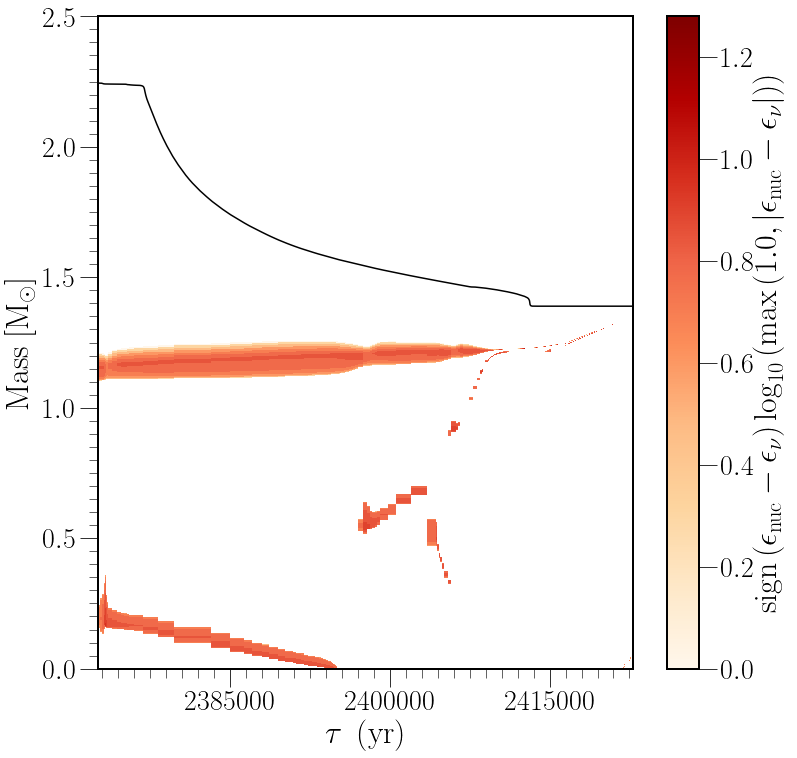
\includegraphics[width=0.5\textwidth]{Kip_m1.png} &
  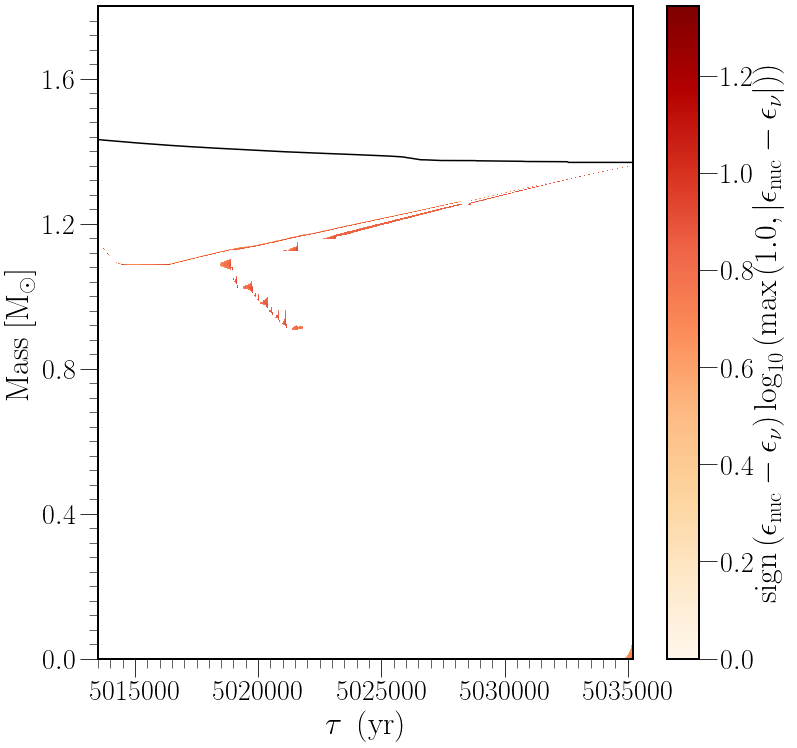
\includegraphics[width=0.5\textwidth]{Kip_m2.png} \\
  \end{array}$
  \caption{}
  \label{fig:1}
\end{figure*}


\subsection{Late evolution and thermonuclear runaway}
\begin{figure*}[htb!]
\begin{center}
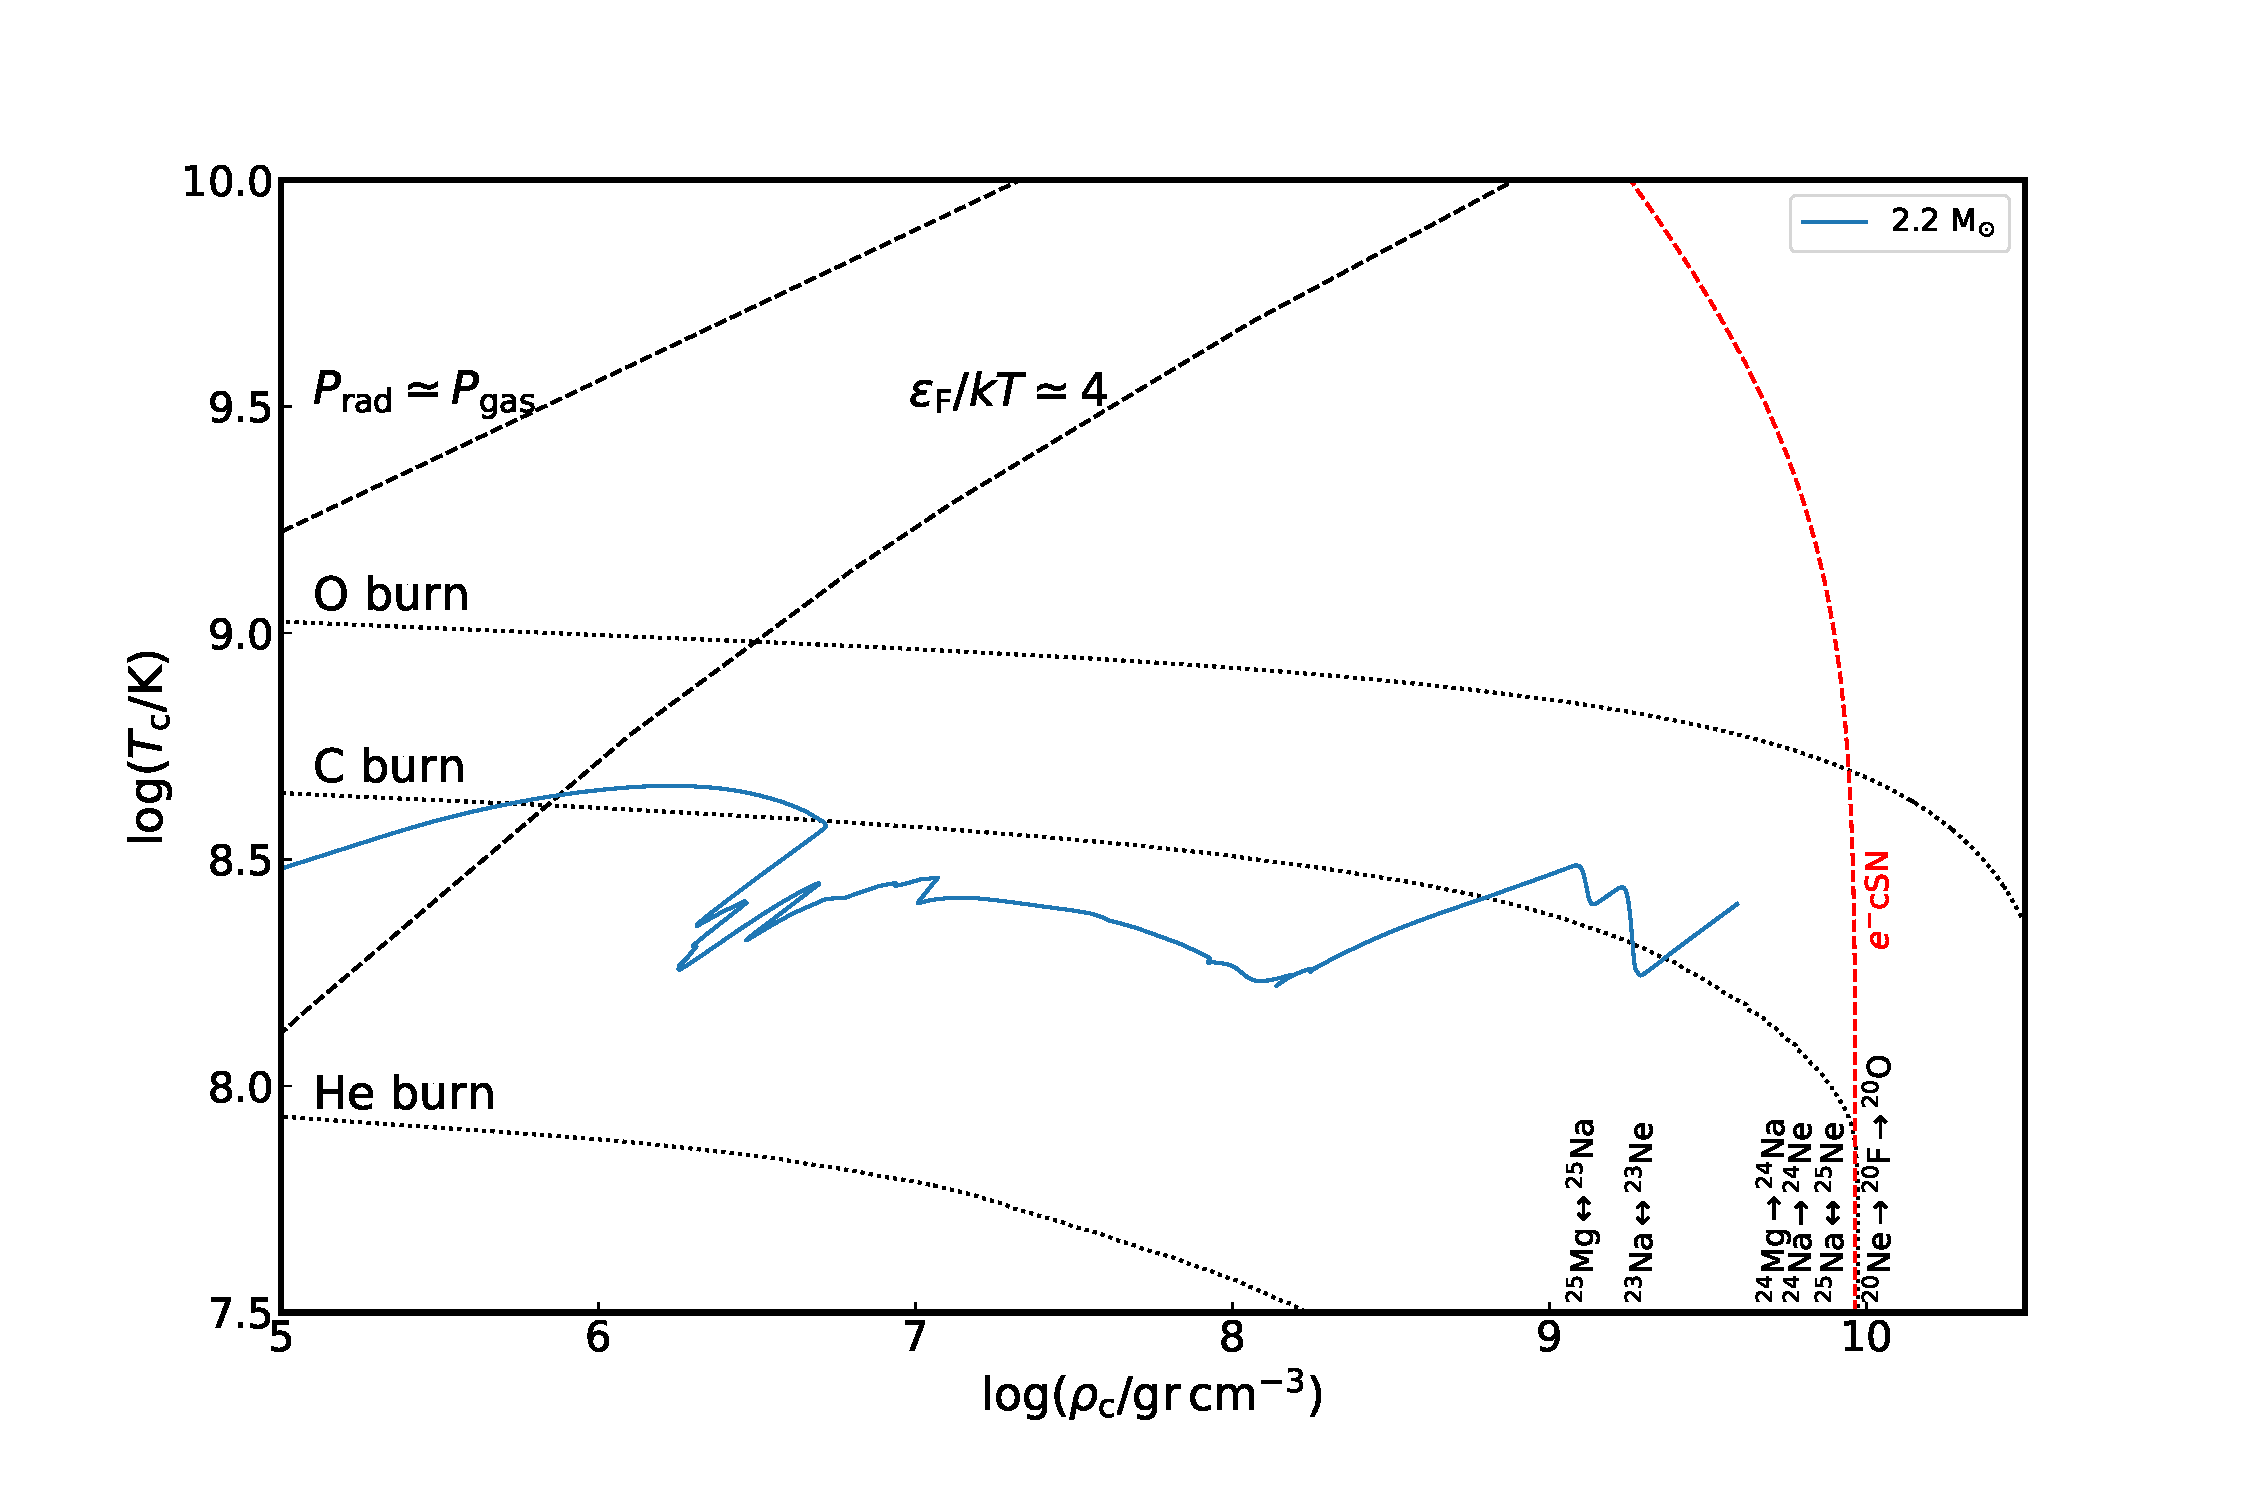
\includegraphics[width=1.0\textwidth]{Rhoc_vs_Tc.pdf}
\caption{Evolution of the core density and temperature }
\label{fig:2}
\end{center}
\end{figure*}



\section{Energetics and nucleosynthesis}\label{sec:3}
some text
\begin{figure}[htb!]
\begin{center}
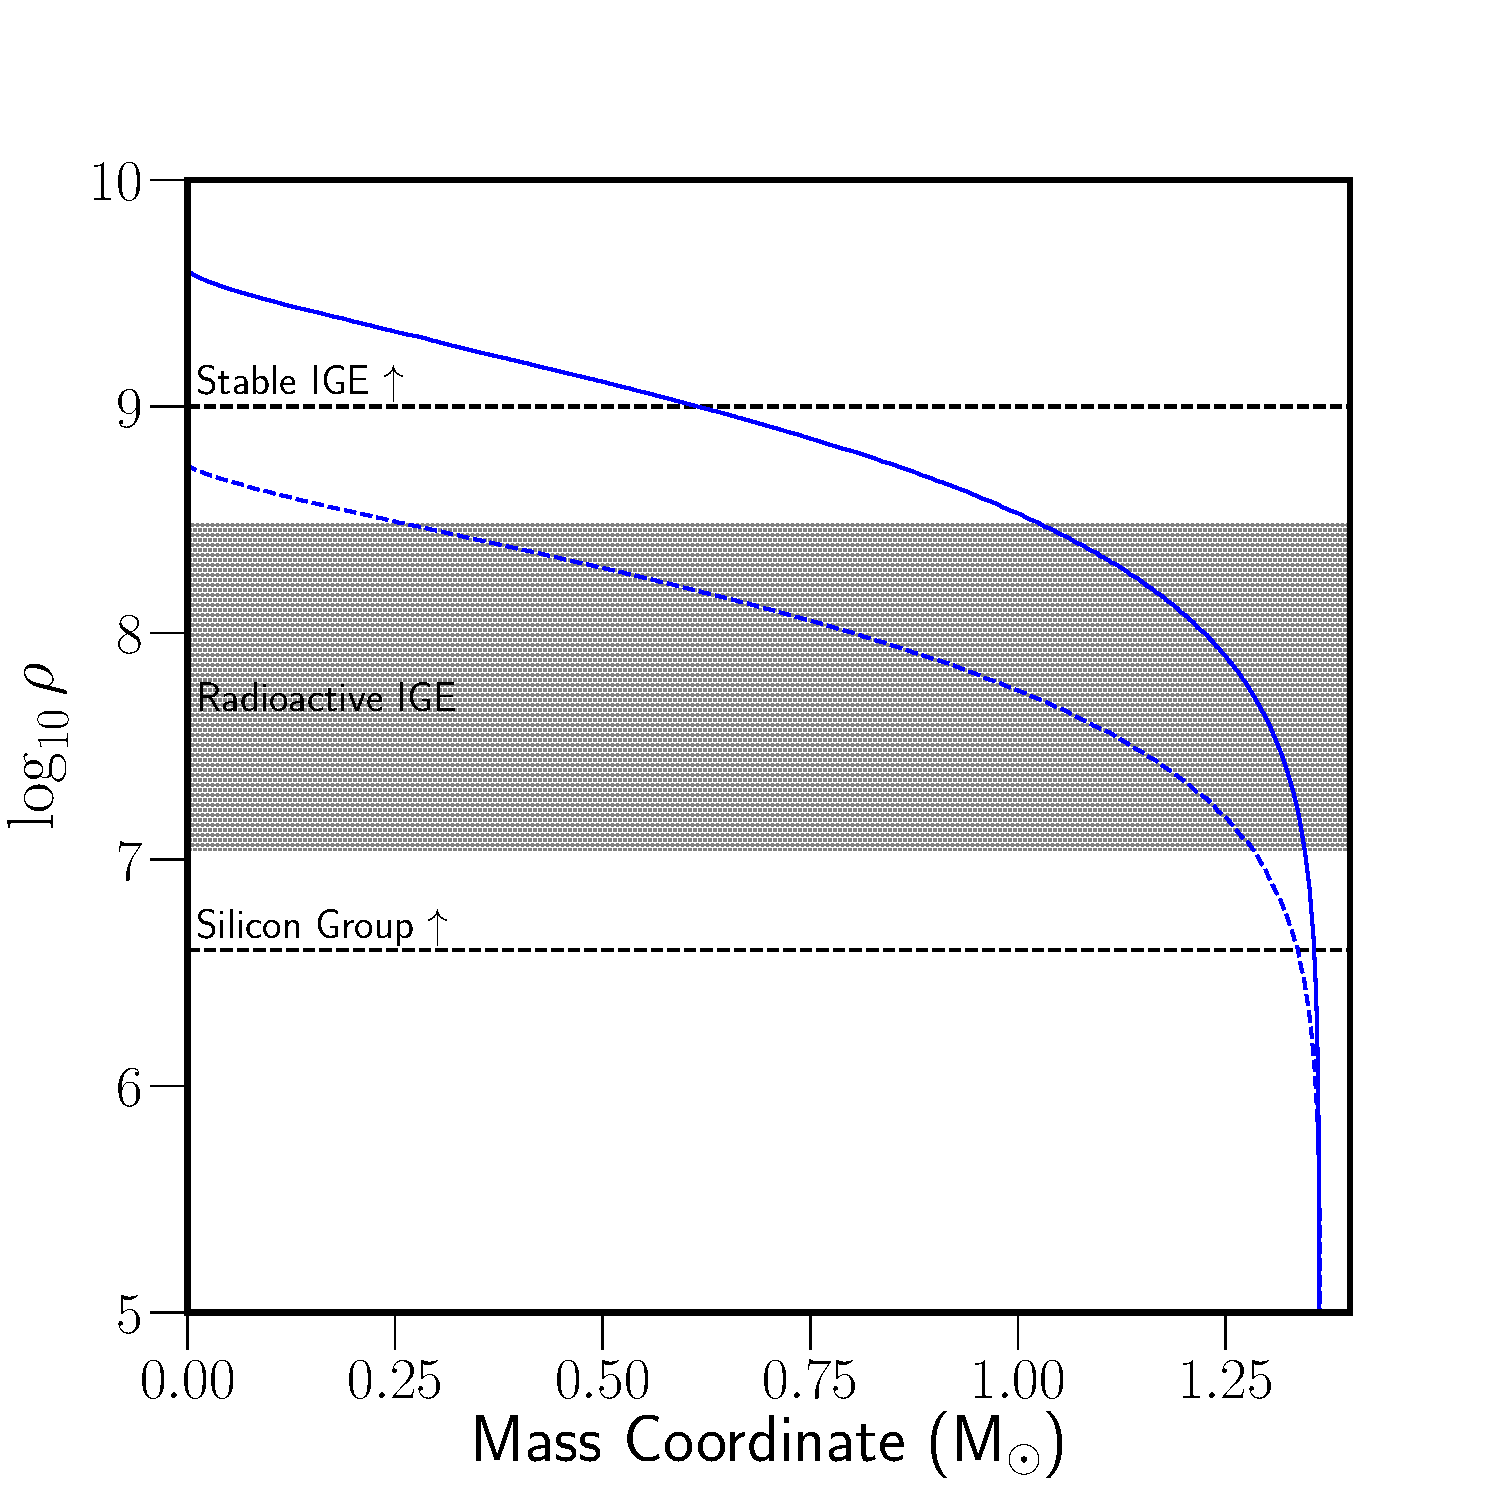
\includegraphics[width=0.5\textwidth]{nucleosynthesis.pdf}
\caption{Density profiles}
\label{fig:nuc}
\end{center}
\end{figure}


\section{Rates and delay times}\label{sec:4}
A useful proxy for the potential \one/\ia connection would be a comparison between 
the \ia occurrence rate, n$_{\rm \ia}$, and the number of stripped  near-Chandrasekhar mass \one cores, $n_\star$.  Here, we provide a simple estimate based
on first principles to demonstrate that the two may indeed be similar. 

Starting with a stellar population of a given mass, to first order, $n_\star$ would be some fraction of the stars that will end up forming   \one cores. Since the hydrogen envelope needs to be removed before the onset of core helium burning, these stars would also need to be members of close  binary systems, thus:  
\begin{equation}
n_{\star} \simeq  f_{\rm bin} \times f_{\rm int} \times  n_{\rm \one}.
\end{equation}
Here, $f_{\rm bin}\simeq 0.7$ \citep{Sana:2012px} is the stellar binary fraction,   $n_{\rm \one}$ is the total 
number of stars with \one cores, and $f_{\rm int}\leq 1$ is an efficiency factor to account for the impact of binary interactions (see below).
\begin{figure*}[htb!]
\begin{center}
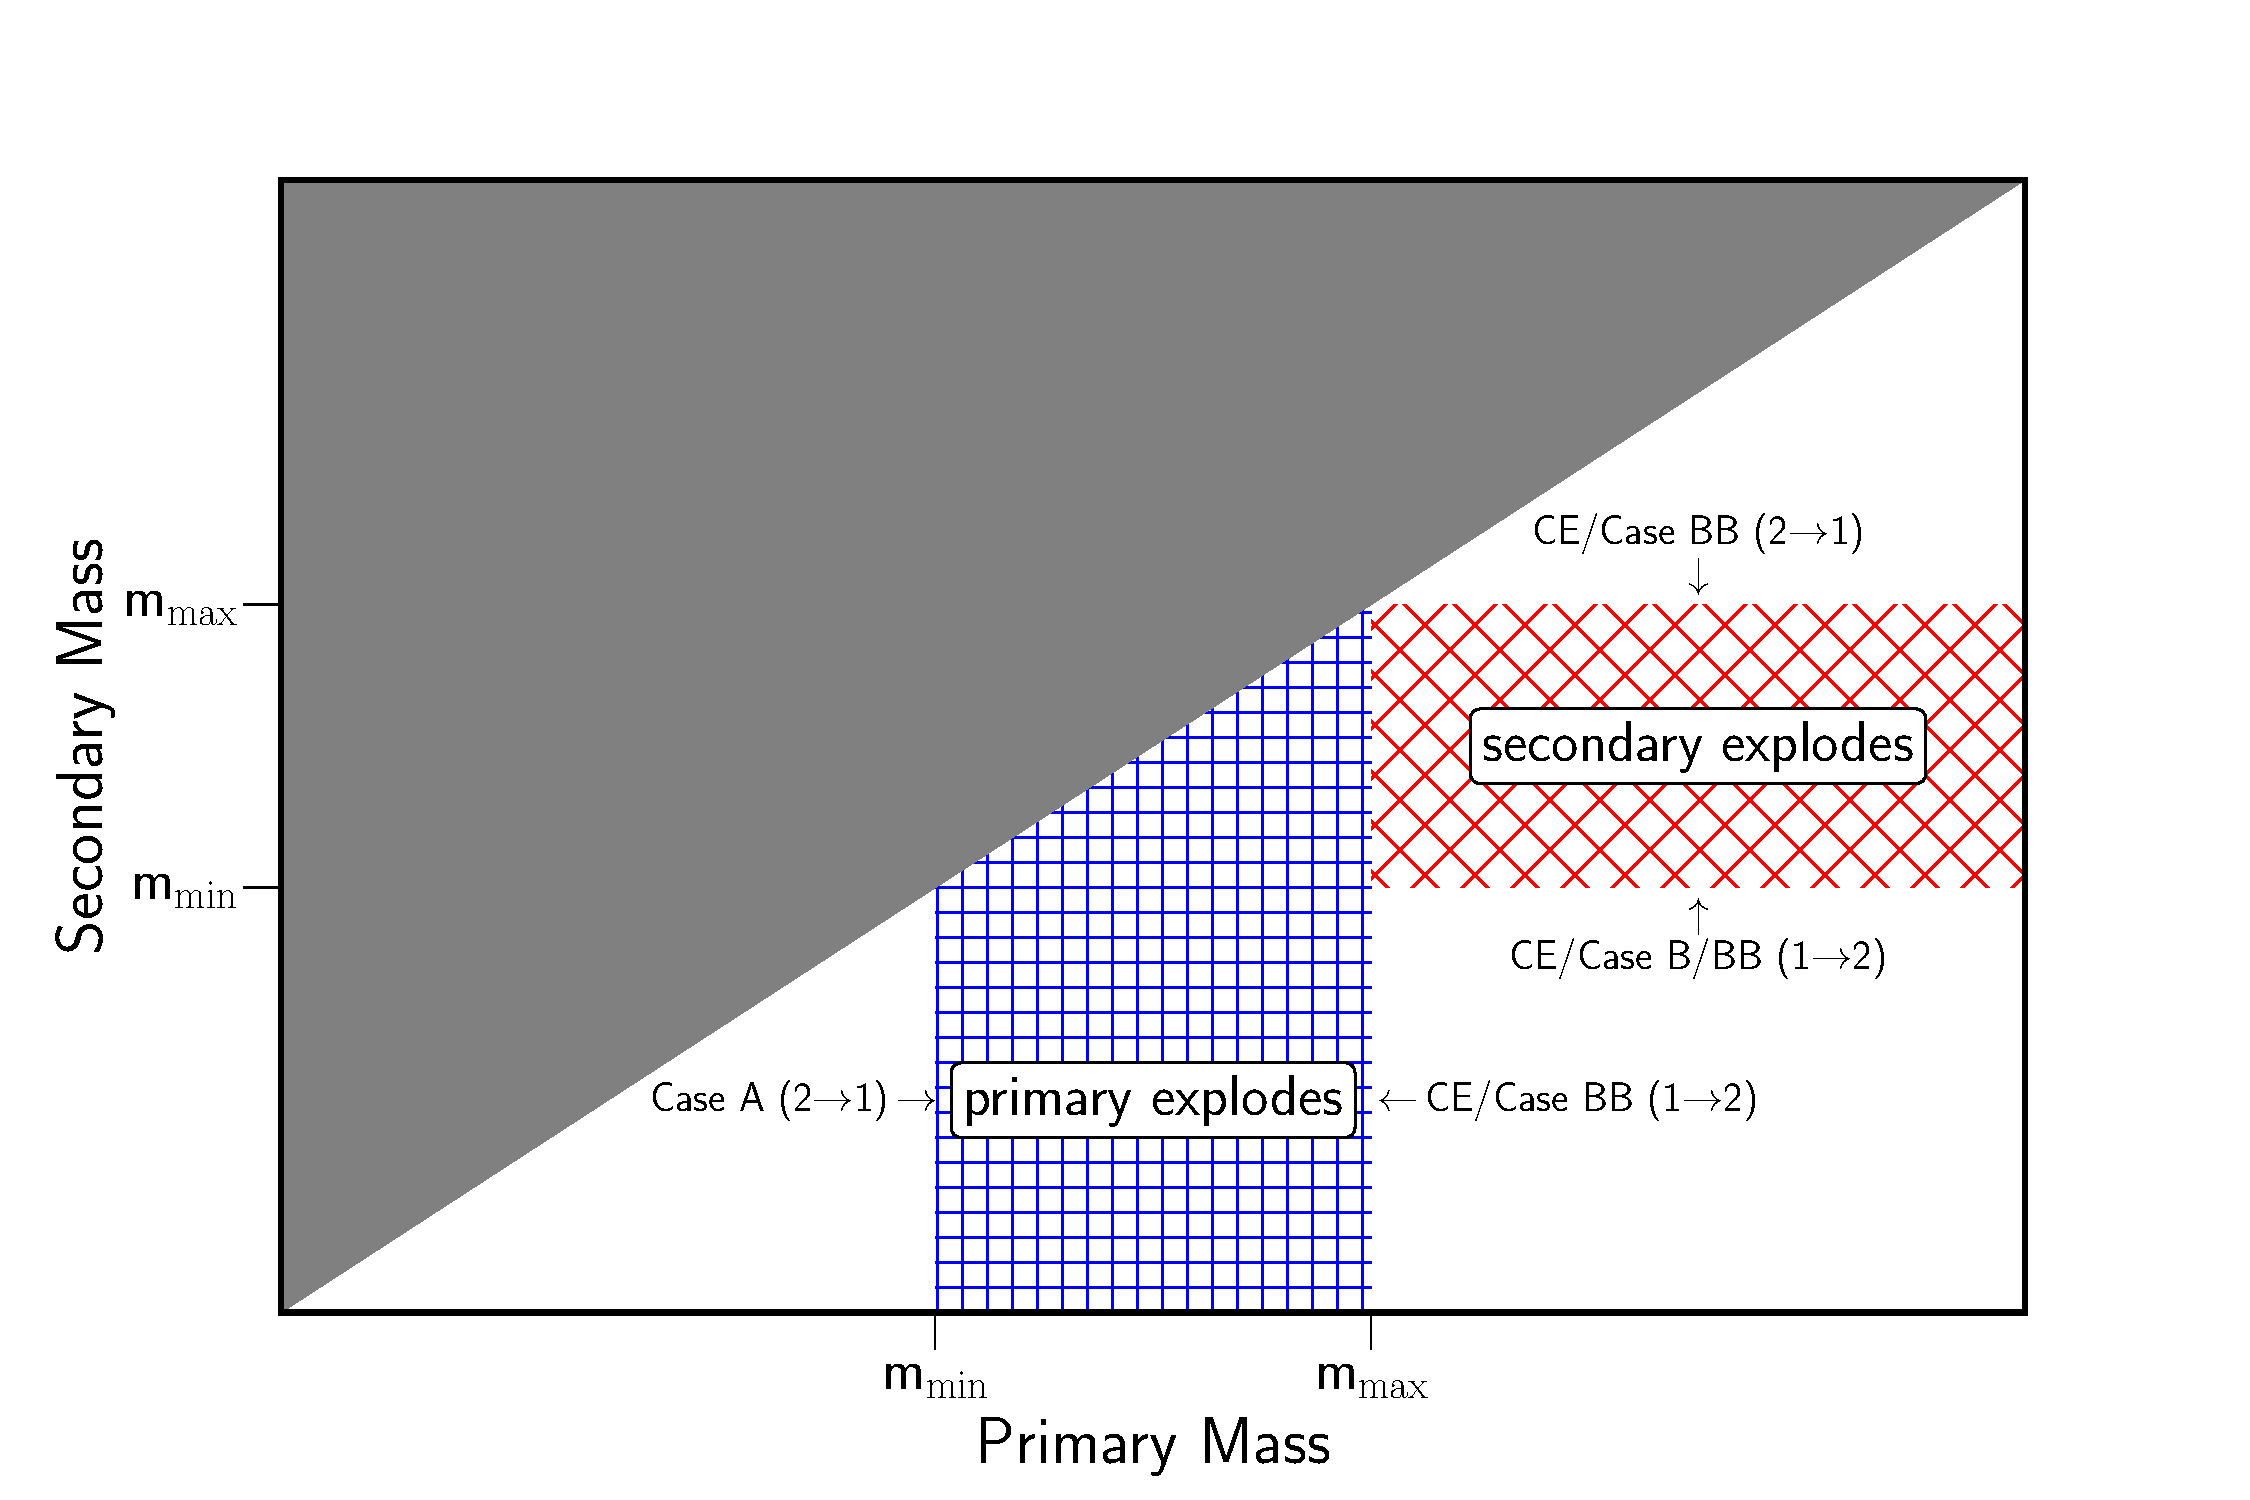
\includegraphics[width=1\textwidth]{formation_regimes.pdf}
\caption{Evolution of core density and temperature }
\label{fig:rates}
\end{center}
\end{figure*}
For binaries, the number of systems with ZAMS masses within a certain range (Figure\,\ref{fig:rates}) is:
\begin{equation}
n(m_1,m_2)dm_1dm_2 = m_1^{\alpha}q^{\kappa}dm_1dq,
\end{equation}
where $m_1$ is the mass of the primary, here defined as the initially more massive star, 
$q\equiv m_2/m_1\leq 1$ is the mass ratio, and $a,\kappa$ depend on the 
initial mass function (IMF) and mass-ratio distribution respectively. Integrating, one finds:
\begin{equation}\label{eq:3}
\begin{split}
N =  
\iint\limits_{m_{\rm min}\,q_{1}}^{m_{\rm max}\,q_{2}}m_1^{\alpha}q^{\kappa}dm_1dq  
 = f\frac{(m_{\rm min}^{\alpha+1} - m_{\rm max}^{\alpha+1})(q_{1}^{\kappa+1} -  q_{2}^{\kappa+1})}{(\alpha+1)(\kappa+1)}, 
\end{split}
\end{equation}
where $f$ is an appropriate normalization factor. 
Naively, one would expect the largest contribution from stars able to evolve
to the SAGB in isolation, viz. stars with ZAMS masses between $\sim 7$ and 11\msun\ \citep{Farmer:2015afs}. 
Since accretion from a companion is not required to trigger an explosion, 
both primaries and secondaries (namely \emph{all} 7--11\msun\ stars formed in binaries) 
can contribute to $n_\star$. Hence, one finds $(m_{\rm min},m_{\rm max})=(7,11)\msun;(q_1,q_2)=(0,1)$ for the primaries (blue region in 
Figure\,\ref{fig:rates}), and $(m_{\rm min},m_{\rm max})=(11,125)\msun;(q_1,q_2)=(7/11,1)$ for the secondaries (red region). For normalization, we consider all systems within $(m_{\rm min},m_{\rm max})=(0.1,125)\msun$. Adopting a 
\cite{Chabrier:2004vw} IMF with $a=-2.35$ for $m_1 \ge 1$ and a $q-$distribution with $k=-0.1$, as inferred for massive stars \citep{Sana:2012px},
Eq.\,\ref{eq:3} yields $n_{\rm \one}\times f_{\rm bin} \simeq 5.42\times 0.7=0.0039$ stars per solar mass formed, with the largest contribution, $\sim 80\%$ coming from primaries. For $f_{\rm int}\simeq 1$, $n_\star$ would therefore exceed the number of \ia  integrated over a Hubble time, $n_{\rm \ia}\simeq0.0027\msun^{-1}$.

However, $f_{\rm int}$ is most likely smaller than unity. Firstly, only a fraction of 
initial binary population will create naked helium stars. Most  systems within the 
hatched regions of Figure\,\ref{fig:rates} will transfer mass to their less massive 
companions after leaving the main sequence. For most cases, this  process will be 
dynamically unstable, leading to the removal of the envelope, so naively, one would 
expect $f_{\rm int}\gtrsim 0.6$. 

Following the stripping of the envelope, any 
subsequent interaction should be sufficiently delayed, for the core to 
grow substantially in mass. The post-CE orbital period distribution should generally 
favor close binaries. Consequently, only a small fraction of the population will have 
separations $\gtrsim 100\rsun$ to experience a second CE episode. 
Nonetheless, a number of more compact binaries that will undergo stable case BB Roche-lobe 
overflow (RLO), could still leave behind stripped \one cores of sufficiently high mass. For instance, the
binary simulations of \cite{Tauris:2015xra} produce a considerable number of \one proto-WDs 
with $m\simeq \mch$ and practically no helium in their envelopes.  

Considering the domonant uncertainties, one finds $0.2 \lesssim f_{\rm int}\lesssim 0.5$. 
Taking into account further ambiguities in the IMF and initial configurations, we conclude that $0.08\lesssim n_\star / n_{\rm \ia} \lesssim 2$. Unsurprisingly, this is also consistent with the findings of detailed population synthesis studies for the occurrence rate of ECSNe \citep[e.g.][]{Jones:2018ule}

Obviously, the above estimate does not consider all possible ways in 
which  systems could move in and out of the hatched regions in 
Figure\,\ref{fig:rates}. Of particular importance may be interactions 
occurring before the helium-burning phase. For instance, there are  
roughly three times as many systems with a total mass larger than 7\msun\  
than there are stars within the hatched regions of Figure\,\ref{fig:rates}. 
A fraction of this population can contribute to the observed rate via Case A/B RLO. 

Similarly,  additional contributions may come from higher-order multiple systems and dynamical interactions in dense environments (see next section). 

\subsection{Delay Time Distribution}\label{sec:4.2}
Besides the integrated number of \ias, a property that is more challenging to match is the evolution of the \ia rate with Cosmic time. 
The time-dependent \ia rate following a burst of star formation, a.k.a the delay time distribution function, \dtd, is generally modeled as a power law with index  

\section{Discussion}\label{sec:5}
We have shown that stars able to form degenerate \one cores after losing 
their hydrogen rich envelopes to binary interactions, are likely to explode 
as \ias instead of undergoing an ECSN and forming a neutron star
(Sections\,\ref{sec:2} \& \ref{sec:3}). The frequency of these objects is 
sufficiently high to a count for a considerable fraction of the \ia 
occurrence rate (Section\,\ref{sec:4}). 
{\bf G\"{o}tz \& Norbert, would you be able to provide some input about 
MLT+,  winds/velocities and possible WR-like properties of the progenitors?}

\acknowledgments
We thank Philipp Podsiadlowski, Friedrich R\"{o}pke,  Samuel Jones and Josiah Schwab for useful discussions.
%
 This research made extensive use of NASA's ADS.

\software{\textsc{mesa}\footnote{http://mesastar.org} \citep{Paxton:2010ji,Paxton:2013pj,Paxton:2015jva,Paxton:2017eie},
          Astropy\footnote{http://www.astropy.org} \citep{Robitaille:2013mpa,Price-Whelan:2018hus}},
          mesaplot \citep{robert_farmer_2018_1441329}

\bibliography{singleIas} 
\bibliographystyle{yahapj}


\end{document}

